\documentclass[a4paper]{book}
\usepackage{geometry}
\geometry{a4paper, left=3cm, right=3cm, top=3cm, bottom=3cm}

\usepackage[T1]{fontenc}
\usepackage[utf8]{inputenc}
\usepackage[italian]{babel}
\usepackage{caption}
%\usepackage{geometry}
%\usepackage{xcolor}
%\usepackage{quoting}
%\usepackage[colorlinks]{hyperref}
%\hypersetup{hidelinks}
%\usepackage{amsmath}
%\usepackage{esint}
\usepackage{amsfonts} %mettere i numeri arabi nell'indice
%\usepackage{amsthm}
\usepackage{graphicx} %includere immagini nel file
%\usepackage{sidecap}
\usepackage{subfigure}
\usepackage{wrapfig}
%\usepackage{array}
%\usepackage{multirow}
%\usepackage{imakeidx}
\usepackage{hyperref}

\title{Progetto Arduino }
\author{Santacà Samuele \& Faedo Marco }
\date{Anno Accademico 2022-2023}

\begin{document}
	\begin{titlepage}
		\maketitle
	\end{titlepage}
	
	
	%	\frontmatter
	\tableofcontents
	%	\part{Prima parte}
	\chapter{Descrizione}
	blabla
		
	
	\chapter{Componenti}
	%	Questo è il primo capitolo.
	\section{Tabella componenti}
	%	Questa è la prima sezione.
	
	\begin{table}[h]
		\centering
		\begin{tabular}{|c|c|c|}
			\hline
			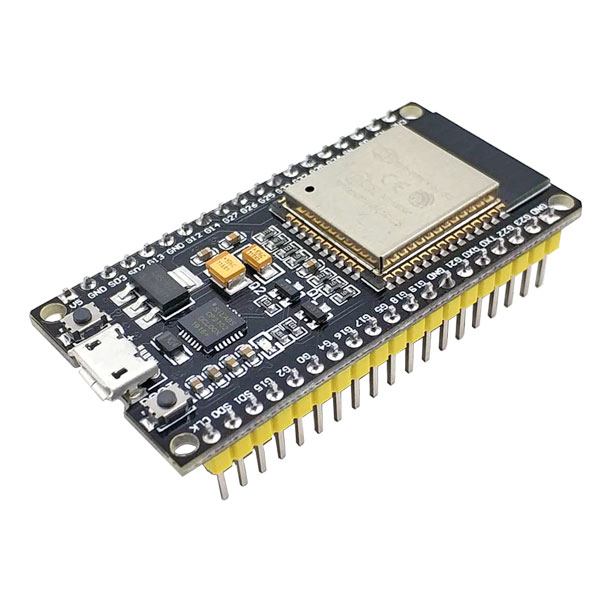
\includegraphics[width=3cm]{C:\Users\Utente\Desktop\uni\corsi_D\Arduino\immagini\esp32.jpg} & \includegraphics[width=3cm]{casa.jpeg} &
			\includegraphics[width=3cm]{immagine3.jpg}\\
			\hline
			\includegraphics[width=3cm]{immagine4.jpg} & \includegraphics[width=3cm]{immagine5.jpg}
			& \includegraphics[width=3cm]{immagine6.jpg} \\
			\hline
			\includegraphics[width=3cm]{immagine7.jpg} & \includegraphics[width=3cm]{immagine8.jpg}
			& \includegraphics[width=3cm]{immagine9.jpg} \\
			\hline
		\end{tabular}
		\caption{Tabella con immagini}
		\label{tab:immagini}
	\end{table}
	
	%\begin{figure}
	%	\subfigure[Prima figura]
	%	{\includegraphics[width=4cm]{casa.jpeg}}
	%	{\includegraphics[width=4cm]{albero.jpg}}
	%	\hspace{1cm}
	%	\subfigure[Terza figura]
	%	{\includegraphics[width=4cm]{castello.jpeg}}
	
	%\end{figure}
	
	%	\begin{figure}
		%		\includegraphics[width=5cm, height=5cm]{albero.jpg} \centering
		%		\caption{didascalia}
		%	\end{figure}
	
	
	
	
	%\begin{figure}
	%	\includegraphics[width=5cm, height=4cm]{albero.jpg}
	%	\caption{didascalia}
	%	\label{nome}
	%\end{figure}
	
	
	\subsection{Descrizione componenti}
	\begin{itemize} %\textbf{parola in grassetto} item=elenco puntato
		\item \textbf{ESP32:} con batteeria da 1.5V con portabatterie per alimentarlo
		\item \textbf{Motori DC:} i motori DC a 3V sono motori a corrente continua che funzionano a una tensione nominale di 3V; hanno un albero di uscita sul quale possono essere installate ruote, ingranaggi, eliche, ecc., per la trasmissione del movimento. La velocità e la direzione di rotazione del motore possono essere controllate variando la tensione applicata alle sue terminazioni.
		\item \textbf{Controllo motori Ponte-H L298N:}
		\item \textbf{Led rosso:}
		\item \textbf{Sensore accelerometro a 3 assi:}
		\item \textbf{Breadboard da 170 punti:}
		\item \textbf{Resistenze:}
		\item \textbf{Sensore infrarossi distanza:}
		\item \textbf{Ruote}:
	\end{itemize}
	
	
	
	%	Questa è la prima sottosezione.
	%	\paragraph{Primo paragrafo}
	%	Questo è un paragrafo.
	
		\chapter{Codice del progetto}
	
	
	\chapter{Collegamenti fisici}
	
	\chapter{Collegamenti esterni}
	
	
	\chapter{Gestione del testo}
	\section{Capoversi}
	\subsection{Metodi di creazione}
	\subsubsection{Metodo 1:}
	Il \emph{capoverso}\index{capoverso} segnala l'inizio di un nuovo argomento.
	
	Questo è un capoverso generato saltando una riga nell'editor.
	\subsubsection{Metodo 2:}
	Il capoverso segnala l'inizio di un nuovo argomento.
	\par Questo è un capoverso generato con l'utilizzo del comando \textbf{$\backslash$par}.
	
	
	
	
	
	
	
	
	
	
	
	
	
	
	
	
	
	
	
	
	
	
	
	
	
	
	
	
	
	
	
	
	
	
	
\end{document}
